\documentclass{standalone}
\usepackage{tikz}
\usetikzlibrary{patterns, positioning}


\begin{document}
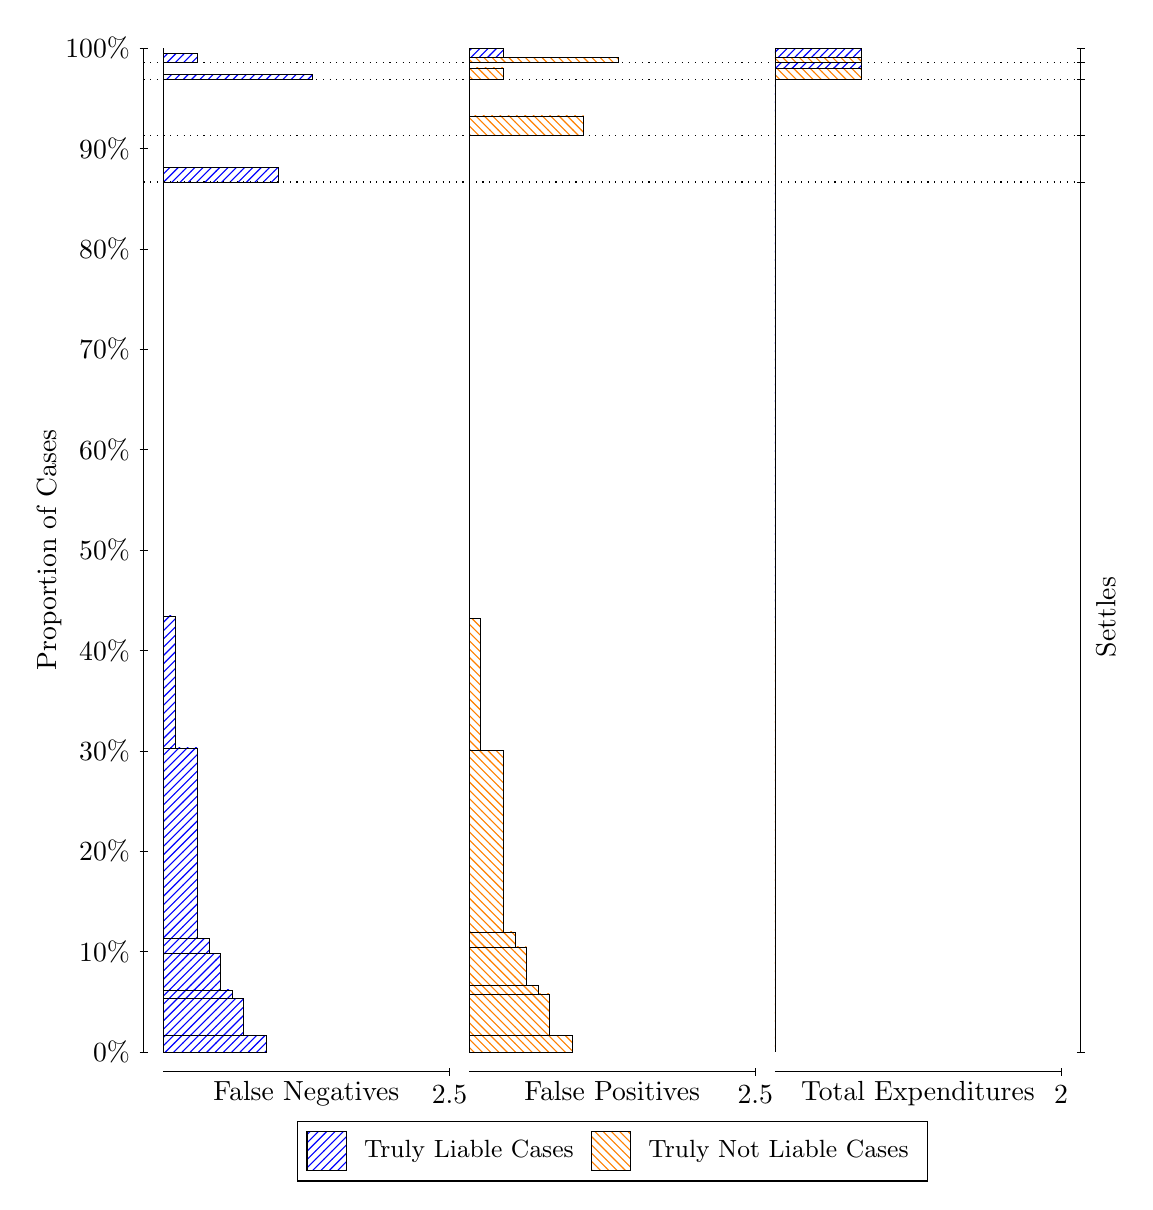
\begin{tikzpicture}
\draw[black, very thin] (1.5,1.75) -- (1.5,14.5);
\node[rotate=90, text=black, anchor=center] at (0.3, 8.125) {Proportion of Cases};
\draw[black, very thin] (1.45,1.75) -- (1.55,1.75);
\node[text=black, anchor=east] at (1.45, 1.75) {0\%};
\draw[black, very thin] (1.45,3.025) -- (1.55,3.025);
\node[text=black, anchor=east] at (1.45, 3.025) {10\%};
\draw[black, very thin] (1.45,4.3) -- (1.55,4.3);
\node[text=black, anchor=east] at (1.45, 4.3) {20\%};
\draw[black, very thin] (1.45,5.575) -- (1.55,5.575);
\node[text=black, anchor=east] at (1.45, 5.575) {30\%};
\draw[black, very thin] (1.45,6.85) -- (1.55,6.85);
\node[text=black, anchor=east] at (1.45, 6.85) {40\%};
\draw[black, very thin] (1.45,8.125) -- (1.55,8.125);
\node[text=black, anchor=east] at (1.45, 8.125) {50\%};
\draw[black, very thin] (1.45,9.4) -- (1.55,9.4);
\node[text=black, anchor=east] at (1.45, 9.4) {60\%};
\draw[black, very thin] (1.45,10.675) -- (1.55,10.675);
\node[text=black, anchor=east] at (1.45, 10.675) {70\%};
\draw[black, very thin] (1.45,11.95) -- (1.55,11.95);
\node[text=black, anchor=east] at (1.45, 11.95) {80\%};
\draw[black, very thin] (1.45,13.225) -- (1.55,13.225);
\node[text=black, anchor=east] at (1.45, 13.225) {90\%};
\draw[black, very thin] (1.45,14.5) -- (1.55,14.5);
\node[text=black, anchor=east] at (1.45, 14.5) {100\%};

\draw[black, very thin] (13.4,1.75) -- (13.4,14.5);
\draw[black, very thin] (13.35,1.75) -- (13.45,1.75);
\node[anchor=west] at (13.35, 1.75) {};
\draw[black, very thin] (13.35,12.798) -- (13.45,12.798);
\node[anchor=west] at (13.35, 12.798) {};
\draw[black, very thin] (13.35,13.393) -- (13.45,13.393);
\node[anchor=west] at (13.35, 13.393) {};
\draw[black, very thin] (13.35,14.102) -- (13.45,14.102);
\node[anchor=west] at (13.35, 14.102) {};
\draw[black, very thin] (13.35,14.313) -- (13.45,14.313);
\node[anchor=west] at (13.35, 14.313) {};
\draw[black, very thin] (13.35,14.5) -- (13.45,14.5);
\node[anchor=west] at (13.35, 14.5) {};

\draw[black, very thin, pattern color=blue, pattern=north east lines] (1.75,1.75) rectangle (3.058,1.9604);
\draw[black, very thin, pattern color=blue, pattern=north east lines] (1.75,1.9604) rectangle (2.7673,2.4332);
\draw[black, very thin, pattern color=blue, pattern=north east lines] (1.75,2.4332) rectangle (2.622,2.5386);
\draw[black, very thin, pattern color=blue, pattern=north east lines] (1.75,2.5386) rectangle (2.4767,3.0003);
\draw[black, very thin, pattern color=blue, pattern=north east lines] (1.75,3.0003) rectangle (2.3313,3.1902);
\draw[black, very thin, pattern color=blue, pattern=north east lines] (1.75,3.1902) rectangle (2.186,5.6113);
\draw[black, very thin, pattern color=blue, pattern=north east lines] (1.75,5.6113) rectangle (1.8953,7.2887);
\draw[black, very thin, pattern color=orange, pattern=north west lines] (1.75,7.2887) rectangle (1.75,12.798);
\draw[black, very thin, pattern color=blue, pattern=north east lines] (1.75,12.798) rectangle (3.2033,12.983);
\draw[black, very thin, pattern color=orange, pattern=north west lines] (1.75,12.983) rectangle (1.75,13.393);
\draw[black, very thin, pattern color=orange, pattern=north west lines] (1.75,13.393) rectangle (1.75,13.637);
\draw[black, very thin, pattern color=blue, pattern=north east lines] (1.75,13.637) rectangle (1.75,14.102);
\draw[black, very thin, pattern color=blue, pattern=north east lines] (1.75,14.102) rectangle (3.6393,14.167);
\draw[black, very thin, pattern color=orange, pattern=north west lines] (1.75,14.167) rectangle (1.75,14.313);
\draw[black, very thin, pattern color=blue, pattern=north east lines] (1.75,14.313) rectangle (2.186,14.435);
\draw[black, very thin, pattern color=orange, pattern=north west lines] (1.75,14.435) rectangle (1.75,14.5);
\draw[black, very thin, pattern color=orange, pattern=north west lines] (5.6333,1.75) rectangle (6.9413,1.9604);
\draw[black, very thin, pattern color=orange, pattern=north west lines] (5.6333,1.9604) rectangle (6.6507,2.4875);
\draw[black, very thin, pattern color=orange, pattern=north west lines] (5.6333,2.4875) rectangle (6.5053,2.593);
\draw[black, very thin, pattern color=orange, pattern=north west lines] (5.6333,2.593) rectangle (6.36,3.0842);
\draw[black, very thin, pattern color=orange, pattern=north west lines] (5.6333,3.0842) rectangle (6.2147,3.2742);
\draw[black, very thin, pattern color=orange, pattern=north west lines] (5.6333,3.2742) rectangle (6.0693,5.5818);
\draw[black, very thin, pattern color=orange, pattern=north west lines] (5.6333,5.5818) rectangle (5.7787,7.2592);
\draw[black, very thin, pattern color=blue, pattern=north east lines] (5.6333,7.2592) rectangle (5.6333,12.798);
\draw[black, very thin, pattern color=orange, pattern=north west lines] (5.6333,12.798) rectangle (5.6333,13.208);
\draw[black, very thin, pattern color=blue, pattern=north east lines] (5.6333,13.208) rectangle (5.6333,13.393);
\draw[black, very thin, pattern color=orange, pattern=north west lines] (5.6333,13.393) rectangle (7.0867,13.637);
\draw[black, very thin, pattern color=blue, pattern=north east lines] (5.6333,13.637) rectangle (5.6333,14.102);
\draw[black, very thin, pattern color=orange, pattern=north west lines] (5.6333,14.102) rectangle (6.0693,14.249);
\draw[black, very thin, pattern color=blue, pattern=north east lines] (5.6333,14.249) rectangle (5.6333,14.313);
\draw[black, very thin, pattern color=orange, pattern=north west lines] (5.6333,14.313) rectangle (7.5227,14.378);
\draw[black, very thin, pattern color=blue, pattern=north east lines] (5.6333,14.378) rectangle (6.0693,14.5);
\draw[black, very thin, pattern color=orange, pattern=north west lines] (9.5167,1.75) rectangle (9.5167,7.2592);
\draw[black, very thin, pattern color=blue, pattern=north east lines] (9.5167,7.2592) rectangle (9.5167,12.798);
\draw[black, very thin, pattern color=orange, pattern=north west lines] (9.5167,12.798) rectangle (9.5167,13.208);
\draw[black, very thin, pattern color=blue, pattern=north east lines] (9.5167,13.208) rectangle (9.5167,13.393);
\draw[black, very thin, pattern color=orange, pattern=north west lines] (9.5167,13.393) rectangle (9.5167,13.637);
\draw[black, very thin, pattern color=blue, pattern=north east lines] (9.5167,13.637) rectangle (9.5167,14.102);
\draw[black, very thin, pattern color=orange, pattern=north west lines] (9.5167,14.102) rectangle (10.607,14.249);
\draw[black, very thin, pattern color=blue, pattern=north east lines] (9.5167,14.249) rectangle (10.607,14.313);
\draw[black, very thin, pattern color=orange, pattern=north west lines] (9.5167,14.313) rectangle (10.607,14.378);
\draw[black, very thin, pattern color=blue, pattern=north east lines] (9.5167,14.378) rectangle (10.607,14.5);
\draw[black, dotted] (1.5,12.798) -- (13.4,12.798);
\draw[black, dotted] (1.5,13.393) -- (13.4,13.393);
\draw[black, dotted] (1.5,14.102) -- (13.4,14.102);
\draw[black, dotted] (1.5,14.313) -- (13.4,14.313);
\draw[black, very thin] (1.75,1.5) -- (5.3833,1.5);
\node[text=black, anchor=north] at (3.5667, 1.5) {False Negatives};
\draw[black, very thin] (5.3833,1.45) -- (5.3833,1.55);
\node[text=black, anchor=north] at (5.3833, 1.45) {2.5};

\draw[black, very thin] (5.6333,1.5) -- (9.2667,1.5);
\node[text=black, anchor=north] at (7.45, 1.5) {False Positives};
\draw[black, very thin] (9.2667,1.45) -- (9.2667,1.55);
\node[text=black, anchor=north] at (9.2667, 1.45) {2.5};

\draw[black, very thin] (9.5167,1.5) -- (13.15,1.5);
\node[text=black, anchor=north] at (11.333, 1.5) {Total Expenditures};
\draw[black, very thin] (13.15,1.45) -- (13.15,1.55);
\node[text=black, anchor=north] at (13.15, 1.45) {2};

\node[text=black, centered, rotate=90] at (13.72, 7.274) {Settles};





\draw (7.449999999999999,1.5) node[draw=none] (baseCoordinate) {};
\begin{scope}[align=center]
        \matrix[scale=0.5, draw=black, below=0.5cm of baseCoordinate, nodes={draw}, column sep=0.1cm]{
            \node[rectangle, draw, minimum width=0.5cm, minimum height=0.5cm, pattern color=blue, pattern=north east lines] {}; &
            \node[draw=none, font=\small, text=black] (B) {Truly Liable Cases}; &
            \node[rectangle, draw, minimum width=0.5cm, minimum height=0.5cm, pattern color=orange, pattern=north west lines] {}; &
            \node[draw=none, font=\small, text=black] (B) {Truly Not Liable Cases}; \\
            };
\end{scope}

\end{tikzpicture}
\end{document}